% Q9: sphere containing a regular square pyramid whose base lies in a great circle.
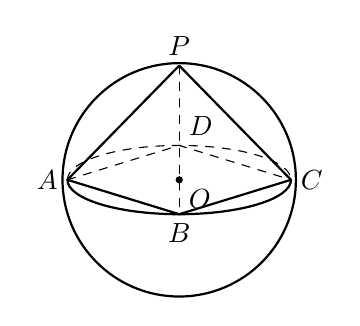
\begin{tikzpicture}[line cap=round,line join=round,x=0.78cm,y=0.78cm]
  \coordinate (O) at (0,0);
  \coordinate (P) at (0,1.86);
  \coordinate (A) at (-1.82,0);
  \coordinate (B) at (0,-0.56);
  \coordinate (C) at (1.82,0);
  \coordinate (D) at (0,0.56);
  \draw[thick] (O) circle (1.9);
  \draw[dashed] (A) arc[start angle=180,end angle=0,x radius=1.82,y radius=0.56];
  \draw[thick] (A) arc[start angle=180,end angle=360,x radius=1.82,y radius=0.56];
  \draw[thick] (A)--(B)--(C);
  \draw[dashed] (A)--(D)--(C);
  \draw[thick] (P)--(A) (P)--(C);
  \draw[dashed] (P)--(B) (P)--(D);
  \fill (O) circle (1.3pt);
  \node[above] at (P) {$P$};
  \node[left] at (A) {$A$};
  \node[below] at (B) {$B$};
  \node[right] at (C) {$C$};
  \node[above right] at (D) {$D$};
  \node[below right] at (O) {$O$};
\end{tikzpicture}
